\documentclass[../part_1.tex]{subfiles}

\begin{document}
\subsection{Обзор существующих аналогов}
\par Современные подходы к извлечению признаковых представлений исходного кода можно условно разделить на две основные категории: специализированные языковые модели для программного кода и универсальные модели, адаптированные для работы с кодом. 
\par Среди наиболее значимых представителей первого направления выделяется CodeBERT\cite{feng2020codebertpretrainedmodelprogramming} -- двуязычная трансформерная модель, разработанная Microsoft Research, которая обучается на парных данных "код-описание" с использованием модифицированных задач маскированного языкового моделирования (\acrshort{mlm}) и обнаружения заменённых токенов (\acrshort{rtd}). 
\par Второе направление ярко представлено моделью UniXcoder\cite{guo2022unixcoder}, которая предлагает унифицированный подход к обработке кода через совместное использование различных модальностей (последовательность токенов, абстрактное синтаксическое дерево и граф потока данных), что позволяет достичь более полного понимания структурных и семантических особенностей программного кода.

\subsubsection{Маскированное языковое моделирование}
\par \acrfull{mlm} -- это ключевая задача предобучения в современных языковых моделях, где модель учится предсказывать специально замаскированные токены в исходном тексте или коде на основе контекста. Этот подход позволяет нейросетям глубоко усваивать синтаксические и семантические зависимости в данных.
% #TODO  Слабо способствует обучению понимания всего кода
\begin{figure}[h]
    \centering
    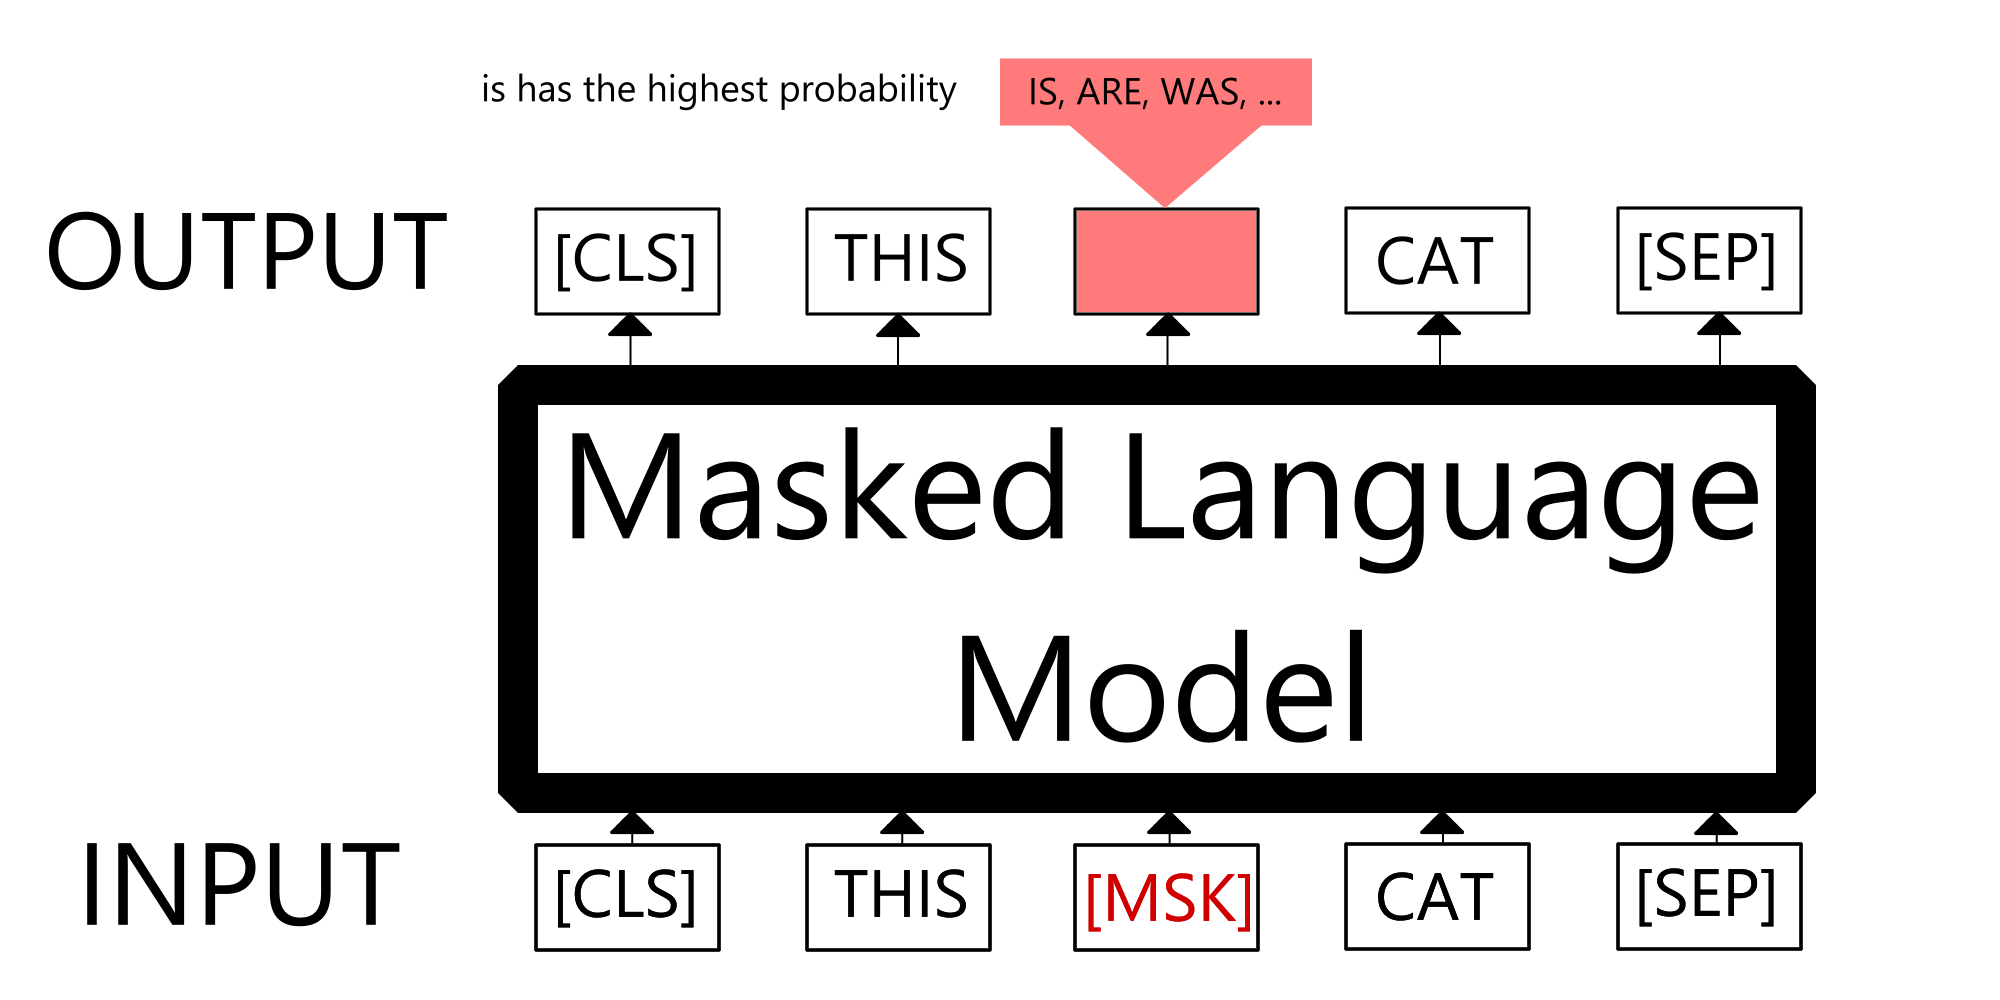
\includegraphics[width=0.8\textwidth]{MLM.png}
    \caption{Пример задачи MLM}
    \label{fig:mlm_bert}
\end{figure}
\par На рисунке \ref{fig:mlm_bert} изображен классический процесс маскированного языкового моделирования. Обучение происходит в 3 шага:
\begin{enumerate}
    \item Маскирование -- выбирается случайное количество токенов. Из них большая часть заменяется на токен [MASK], а оставшиеся либо не меняются, либо заменяются на случайное слово
    \item Предсказание -- модель анализирует контекст вокруг маски и вычисляет вероятность токенов кандидатов.
    \item Функция потерь -- ошибка считается только для замаскированных позиций.
\end{enumerate}
% #TODO Основными приемуществами использованя млм являются
\par Почему же используют \acrshort{mlm}
\begin{itemize}
    \item Контекстное обучение -- модель учится находить взаимосвязи токенов, а не только статистику.
    \item Универасальность -- подходит для любых последовательностей, не требуя разметку.
    \item Подготовка к downstream-задачам -- навык востановления контекста полезно для автопродления текста или же исправления ошибок.
\end{itemize}

\subsubsection{Обнаружения заменённых токенов}
\par \acrfull{rtd} -- это вспомогательная задача предобучения, используемая в современных языковых моделях для более эффективного обучения представлений. 

\begin{figure}[h]
    \centering
    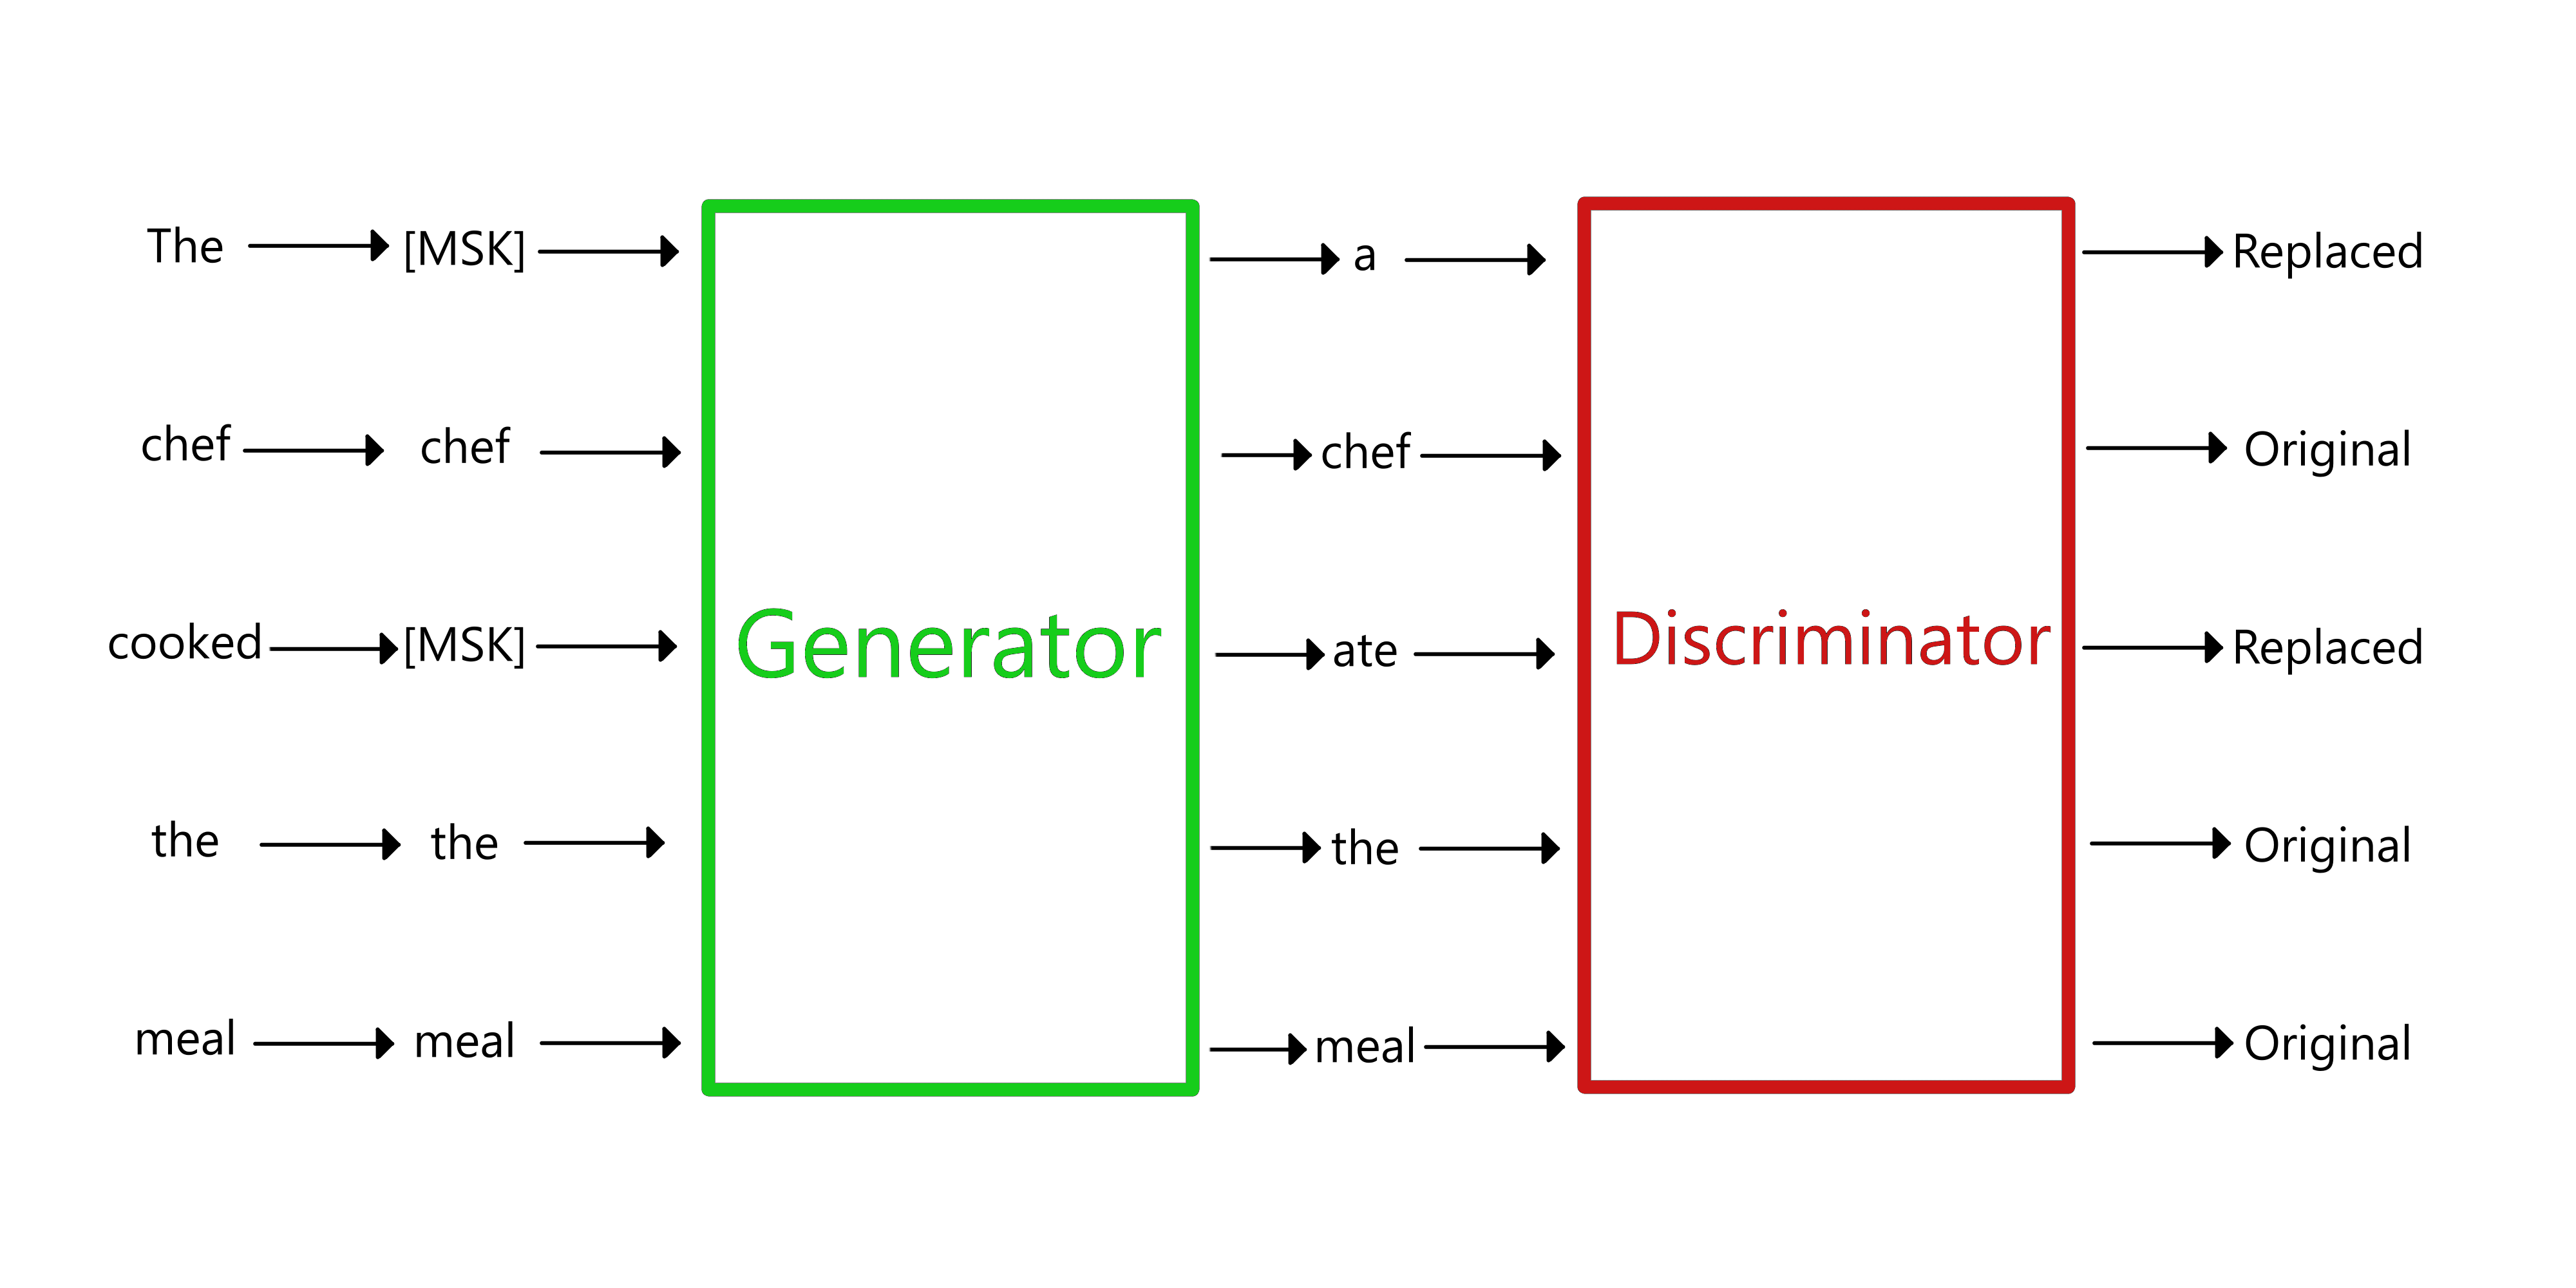
\includegraphics[width=0.6\textwidth]{rtd.png}
    \caption{Пример задачи RTD}
    \label{fig:rtd_bert}
\end{figure}

\par На рисунке \ref{fig:rtd_bert} изображен классический процесс обучения модели на задаче обнаружения заменённых токенов. Обучение происходит в 3 шага:
\begin{enumerate}
    \item Замена токенов -- маленькая модель генератора заменяет токены на новые, схожие по смыслу. К примеру running заменится на jogging 
    \item Предсказание -- модель анализирует контекст вокруг замены выявить является ли токен замененным.
    \item Функция потерь -- ошибка считается для замененных токенов и оригинальных.
\end{enumerate}
% #TODO Основными приемуществами РТД является 
\par Почему же используют \acrshort{rtd}
\begin{itemize}
    % #TODO СПСОБСТВУЕТ ЕЩЕ БОЛЬШЕМУ ПОНИМАНИЮ СТРУКТУРЫ ТЕКСТА
    % #TODO \item Эффективность данных -- все токены используются в момент обучения.
    % #TODO ПЕРЕДЕЛАЙ \item Вычислительная сложность -- низкая у \acrshort{rtd} потому что используется бинарная классификация.
\end{itemize}

\end{document}